\documentclass[sigconf,nonacm]{acmart}

% If acmart unavailable on Overleaf, replace with:
% \documentclass[10pt,twocolumn]{article} and drop the \affiliation block

\settopmatter{printacmref=false, printfolios=false}
\renewcommand\footnotetextcopyrightpermission[1]{}
\pagestyle{plain}

\usepackage{graphicx}
\usepackage{booktabs}
\usepackage{hyperref}
\usepackage{wrapfig}

\setlength{\textfloatsep}{8pt plus 2pt minus 2pt}
\setlength{\intextsep}{8pt plus 2pt minus 2pt}

\title{Project Update: Multi-Modal Performance Sensing for Beach Volleyball Athletes}

\author{Tristan Cooper}
\affiliation{%
  \institution{UC San Diego}
  \city{La Jolla}
  \state{CA}
  \country{USA}
}
\email{tmcooper@ucsd.edu}

\begin{document}
\maketitle

%===================================================================
\section{Problem and Scope Refinement}
%===================================================================

This project builds a multi-modal sensing pipeline that fuses wearable physiology, courtside environmental measurements, and a subjective self-rating to produce per-session factor rankings explaining individual beach volleyball performance variability. Three feedback loops have refined the scope: TA review, three classmate reviews, and a 20-respondent player survey. Two pivots resulted, both directly responsive to TA feedback. \textbf{First}, the subjective 1--10 self-rating has been elevated to the primary outcome; the CV-derived kill/error differential remains in scope but is flagged for demotion to stretch if BalltimeAI access cannot be secured, with the kills/errors-influenced-by-partner-and-opponent limitation to be discussed in the final report. \textbf{Second}, the survey of N=20 players (Section~4) directly informed which contextual features to retain and which to drop, addressing the TA's recommendation to validate user need before further hardware investment.

\begin{figure*}[t]
    \centering
    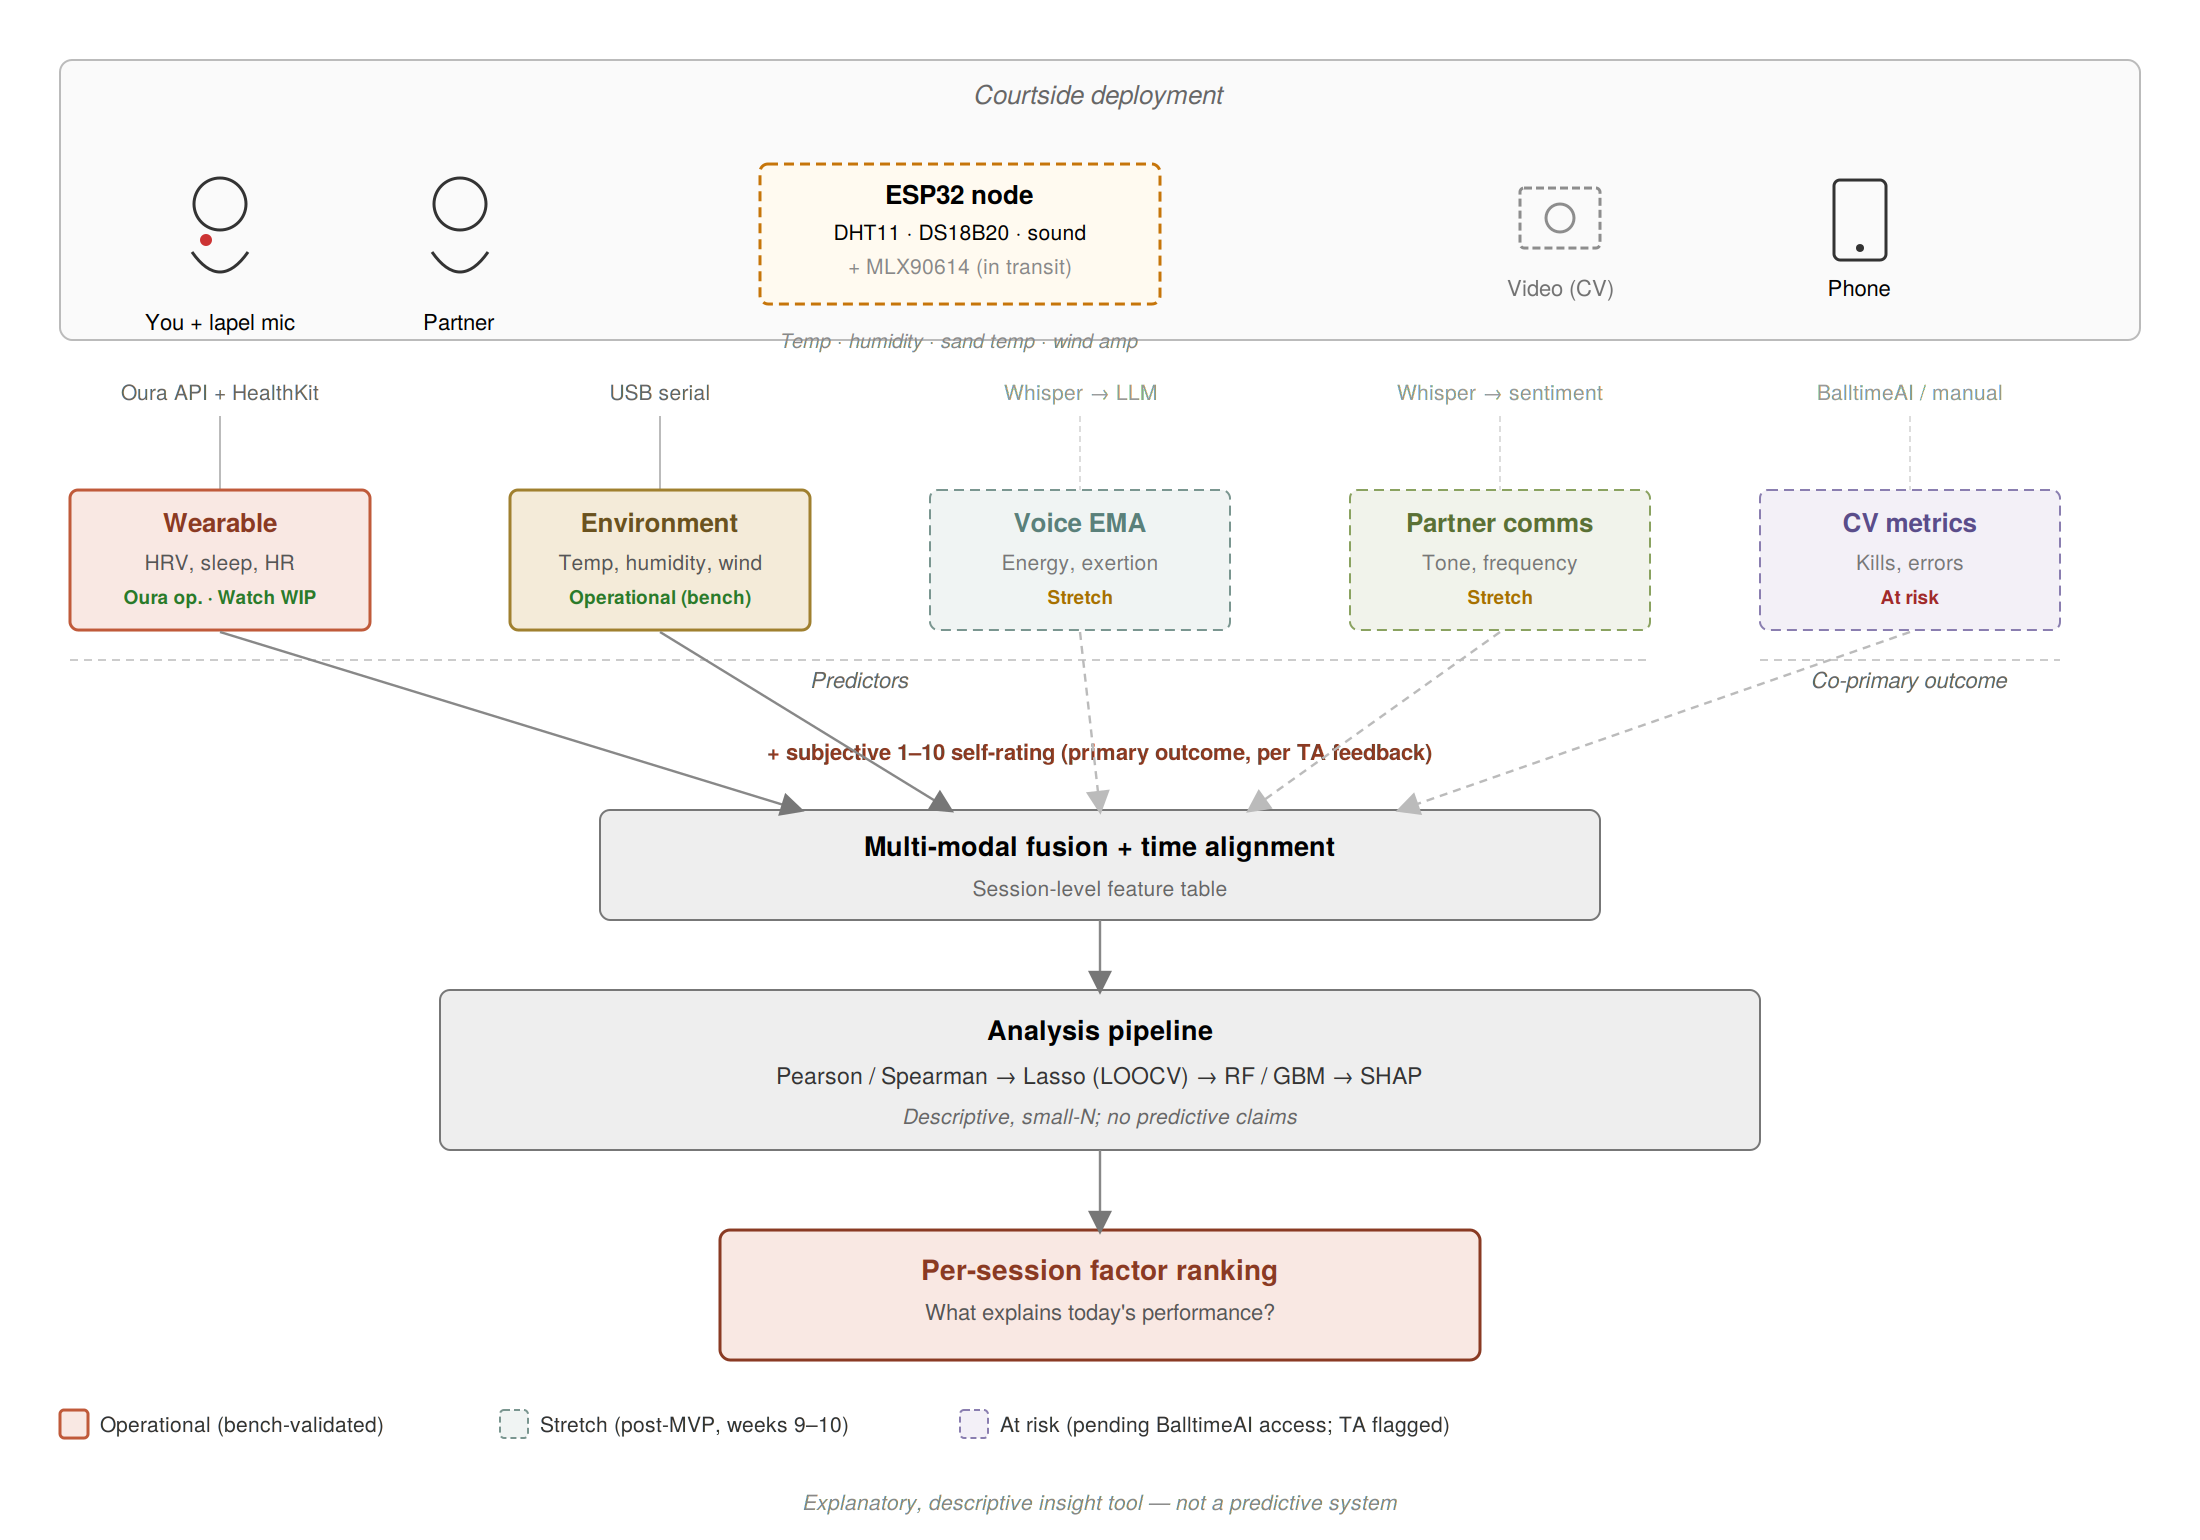
\includegraphics[width=0.92\textwidth]{system_architecture.png}
    \caption{System architecture, annotated with implementation status. Wearable (Oura operational, Apple Watch in progress) and environmental (DHT11 + DS18B20 + sound, MLX90614 in transit) streams are bench-validated. Voice EMA and partner communication are scoped as stretch. The CV outcome is flagged ``at risk'' pending BalltimeAI access per TA feedback on ground-truth quality; the subjective 1--10 self-rating is now the primary outcome.}
    \label{fig:arch}
\end{figure*}

%===================================================================
\section{Hardware Progress}
%===================================================================

The courtside node is built on a Lonely Binary ESP32-S3 with external WiFi antenna. It reads three channels at 0.5~Hz: a DHT11 for ambient temperature and humidity, an analog sound sensor for wind-amplitude estimation, and a DS18B20 waterproof probe as an interim contact-based sand-temperature sensor. An MLX90614 IR thermometer is in transit and will replace the DS18B20 on arrival for non-contact sand-surface measurement. The sound-based wind estimation uses windowed mean-absolute-deviation of the microphone signal as a low-cost intensity proxy; a planned upgrade to an I2S MEMS microphone will be evaluated for better low-frequency response, since wind energy concentrates below 200~Hz and the analog module low-passes aggressively. Anemometer ground truth is acknowledged as a stretch requirement and limitation.

Figure~\ref{fig:hardware} shows the assembled node and a representative bench trace generated by exhaling on the sensor at midpoint, producing the expected coupled spike in temperature ($+0.7^\circ$C) and humidity ($+24\%$ RH) followed by exponential return to ambient --- confirming sensor responsiveness and time-alignment of streams.

\begin{figure}[t]
    \centering
    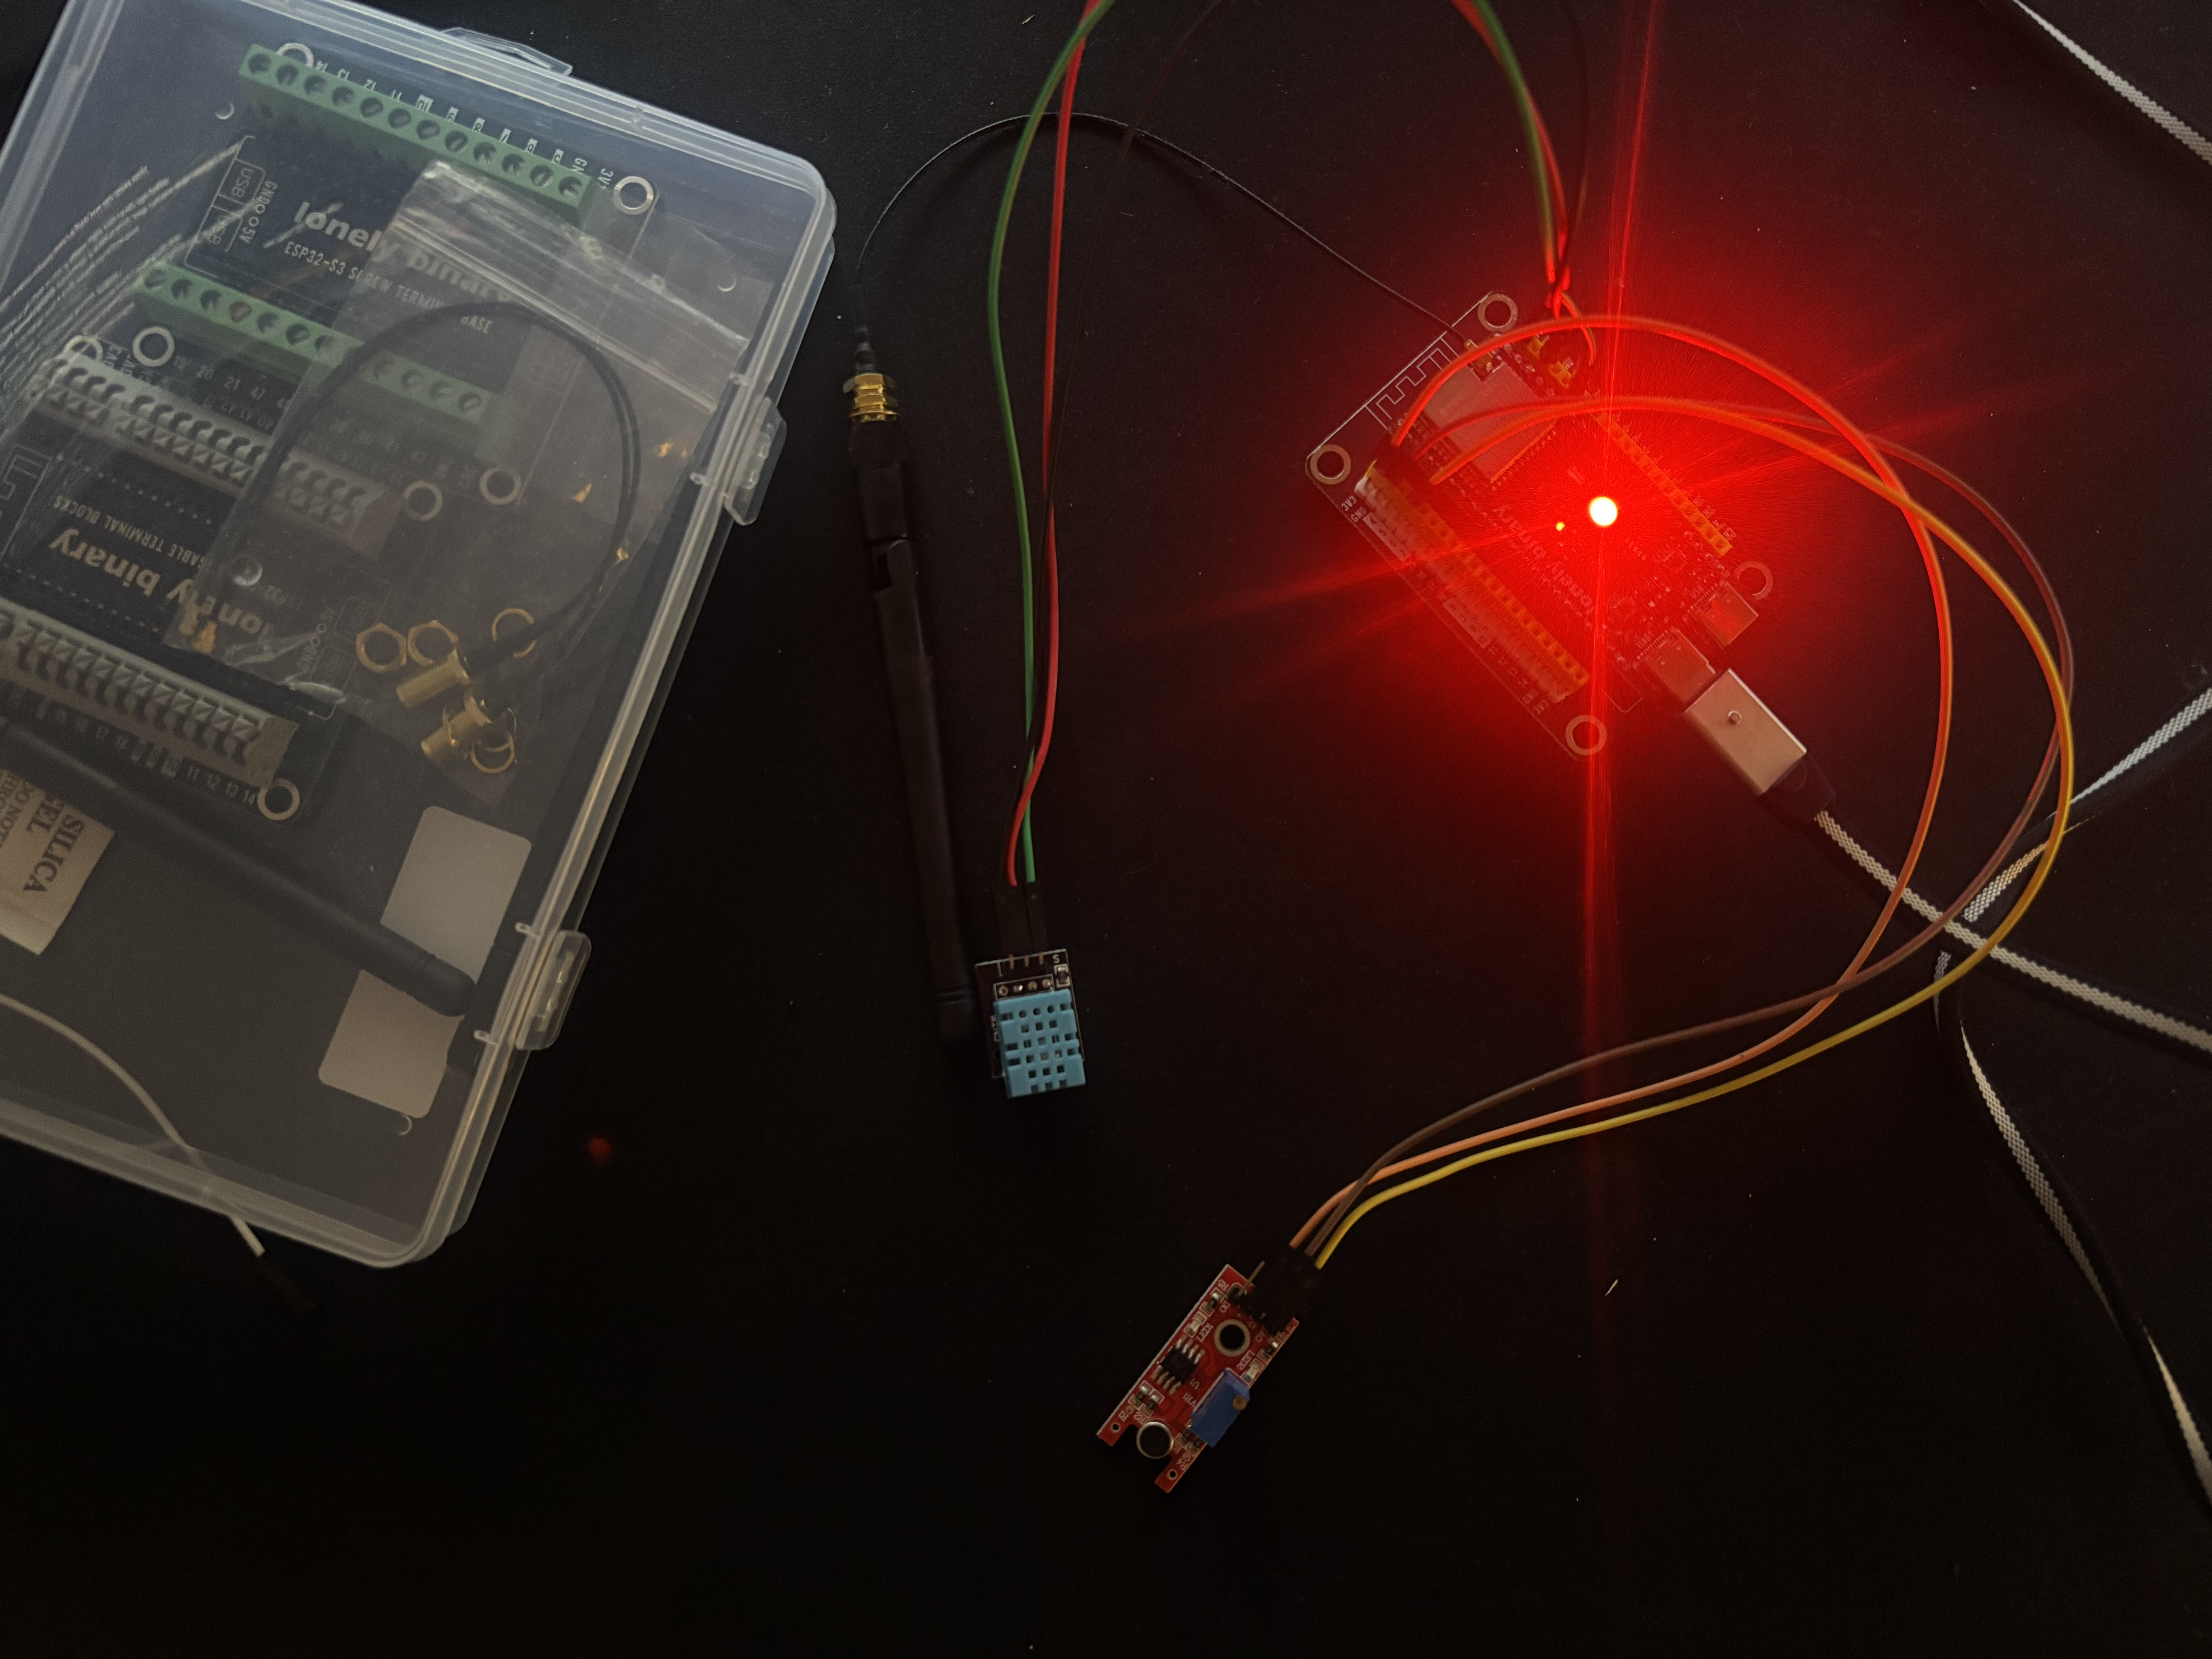
\includegraphics[width=0.43\columnwidth]{hardware_photo.jpg}
    \hfill
    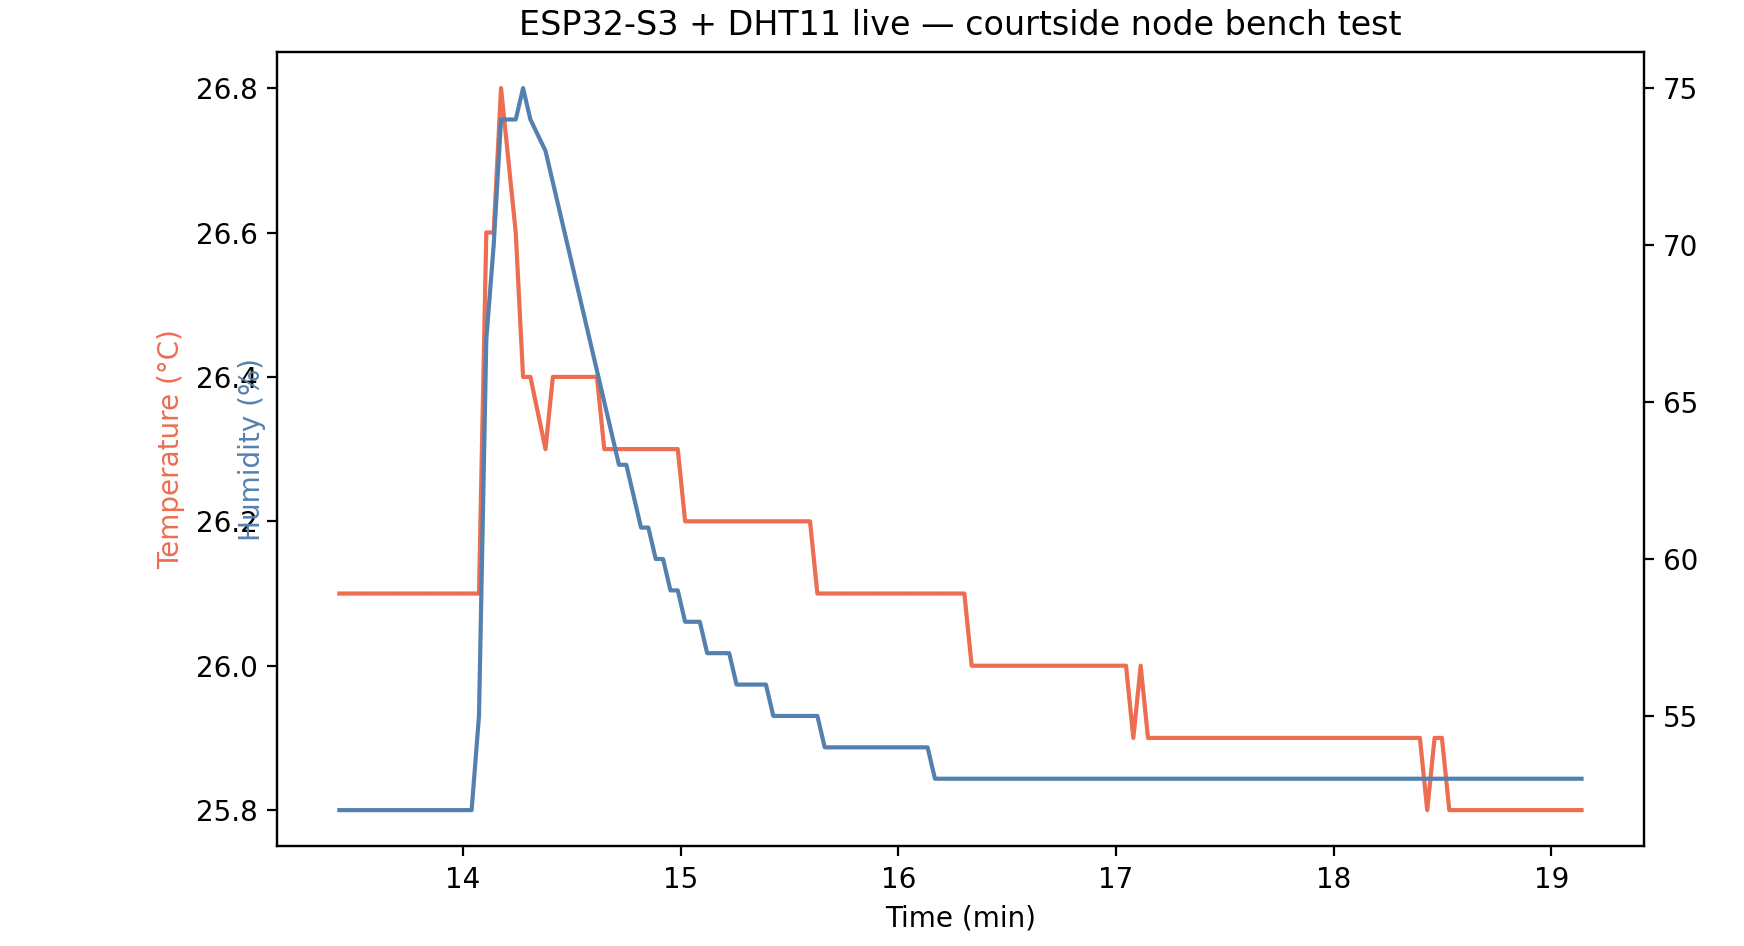
\includegraphics[width=0.55\columnwidth]{esp32_bench.png}
    \caption{Left: assembled ESP32-S3 environmental node with DHT11, sound sensor, and DS18B20 probe. Right: live bench-validation trace with operator exhalation event near $t \approx 14.1$~min producing coupled temperature and humidity response.}
    \label{fig:hardware}
\end{figure}

\begin{figure}[!htbp]
    \centering
    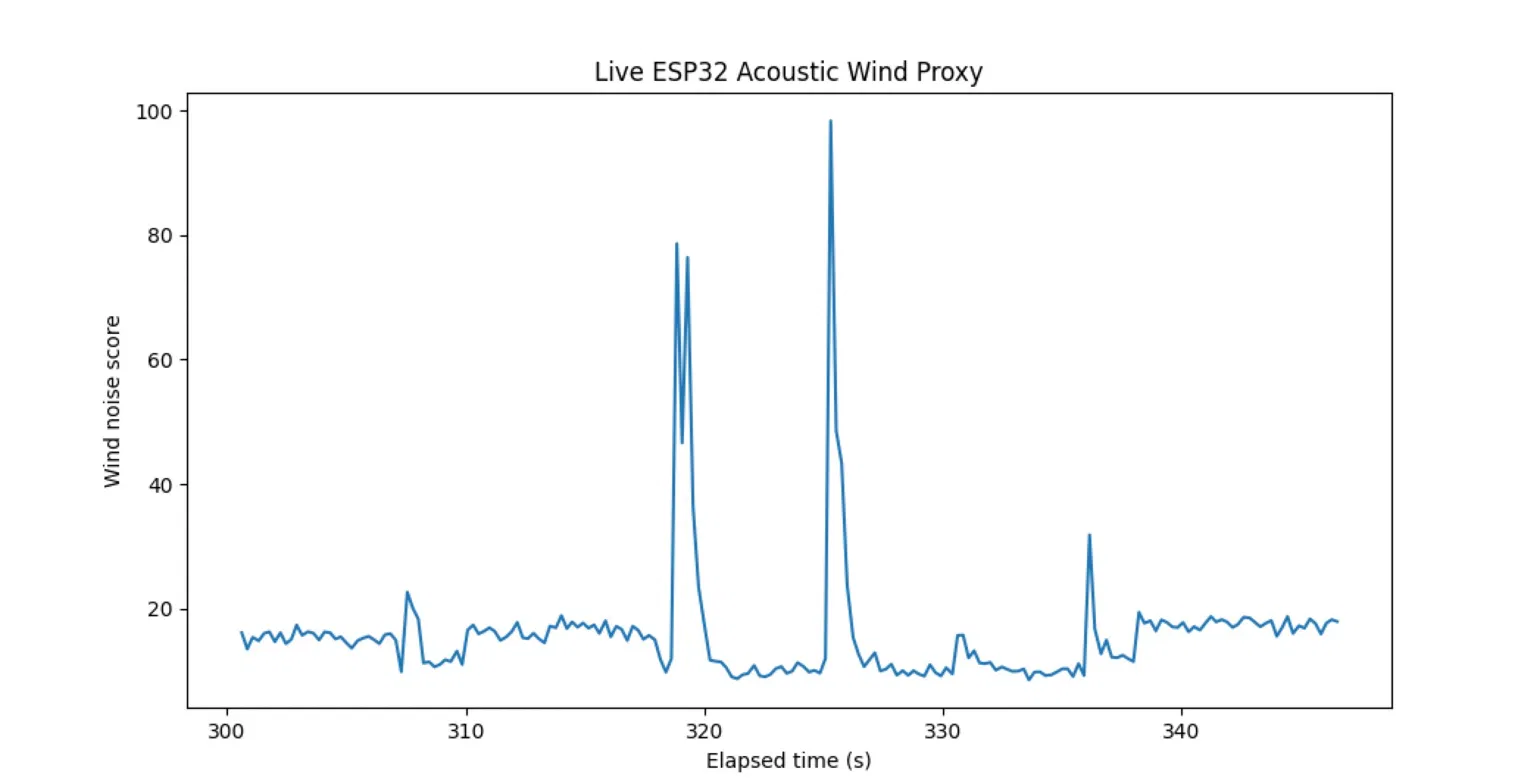
\includegraphics[width=0.98\columnwidth]{wind_proxy.png}
    \caption{First-test validation of the acoustic wind proxy: windowed mean-absolute-deviation of the analog microphone signal. Two large transient spikes near $t = 319$~s and $t = 325$~s are operator-induced (blowing directly on the sensor) and confirm responsiveness; bench ambient baseline is $\sim$15. Quantitative wind-speed calibration against an anemometer remains a stretch goal.}
    \label{fig:wind}
\end{figure}

%===================================================================
\section{Software and Data Pipeline}
%===================================================================

The pipeline is organized as a session-keyed folder structure with one CSV per modality, consolidated downstream into a unified session-level feature table. The ESP32 streams CSV lines over USB serial to a Python bridge that performs live plotting and disk logging in a single pass. Oura integration is complete: a Python client using the v2 personal-access-token API pulls a rolling 21-day window across five endpoints (daily sleep, daily readiness, daily activity, sleep periods, workouts) and writes one normalized CSV per endpoint. Apple Watch via HealthKit export is scoped, not yet implemented; the workflow is a weekly manual export from the iPhone Health app followed by XML parsing of in-session heart rate. Live syncing and a mobile app are explicitly out of scope for this N=1 study --- a researcher-operated workflow is sufficient. Analysis lives in a single Jupyter notebook running the committed pipeline: Pearson/Spearman associations $\to$ Lasso with LOOCV $\to$ random forest and gradient boosting $\to$ SHAP for per-session factor rankings.


\begin{figure}[t]
    \centering
    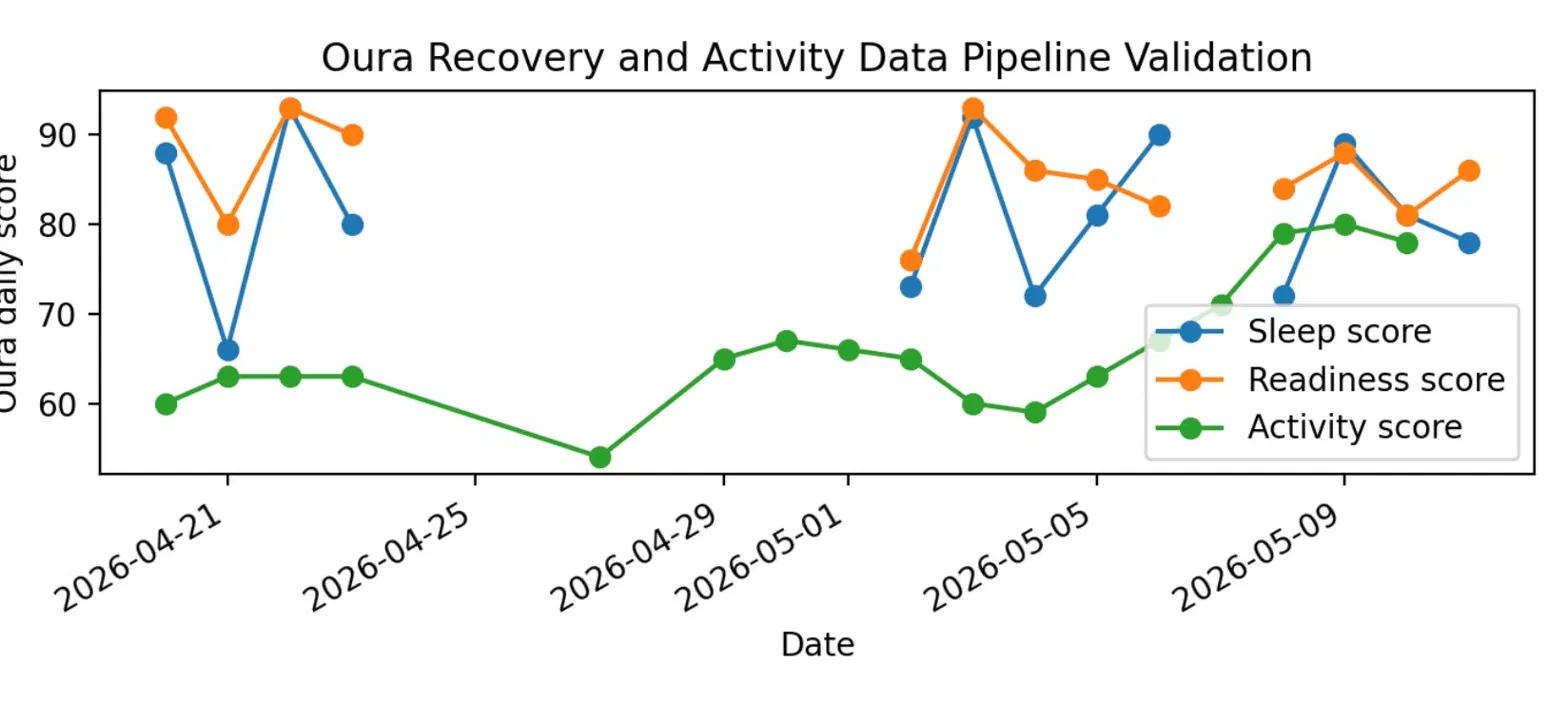
\includegraphics[width=0.98\columnwidth]{oura_validation.png}
    \caption{Oura API pipeline validation: 21-day rolling window of daily sleep, readiness, and activity scores pulled live and normalized to CSV. Activity score reads consistently low because the ring is removed during workouts; the corresponding in-workout activity signal will be filled by the Apple Watch HealthKit pipeline once integrated.}
    \label{fig:oura}
\end{figure}
%===================================================================
\section{User Validation: Player Survey (N = 20)}
%===================================================================

Aggregating responses took longer than anticipated, but the resulting N=20 sample\footnote{Survey link: \url{https://forms.gle/DcEuomBF2MLz8gTh7}} is substantial and reshaped the feature set. Responses came from the UCSD men's and women's beach volleyball teams plus recreational, club, intramural, NCAA, and Open/AVP players outside UCSD; cohort breakdown is shown in Figure~\ref{fig:cohort}. Self-rated skill spanned 1--8 (mean 5.7) on a 10-point scale.

\begin{figure*}[!htbp]
    \centering
    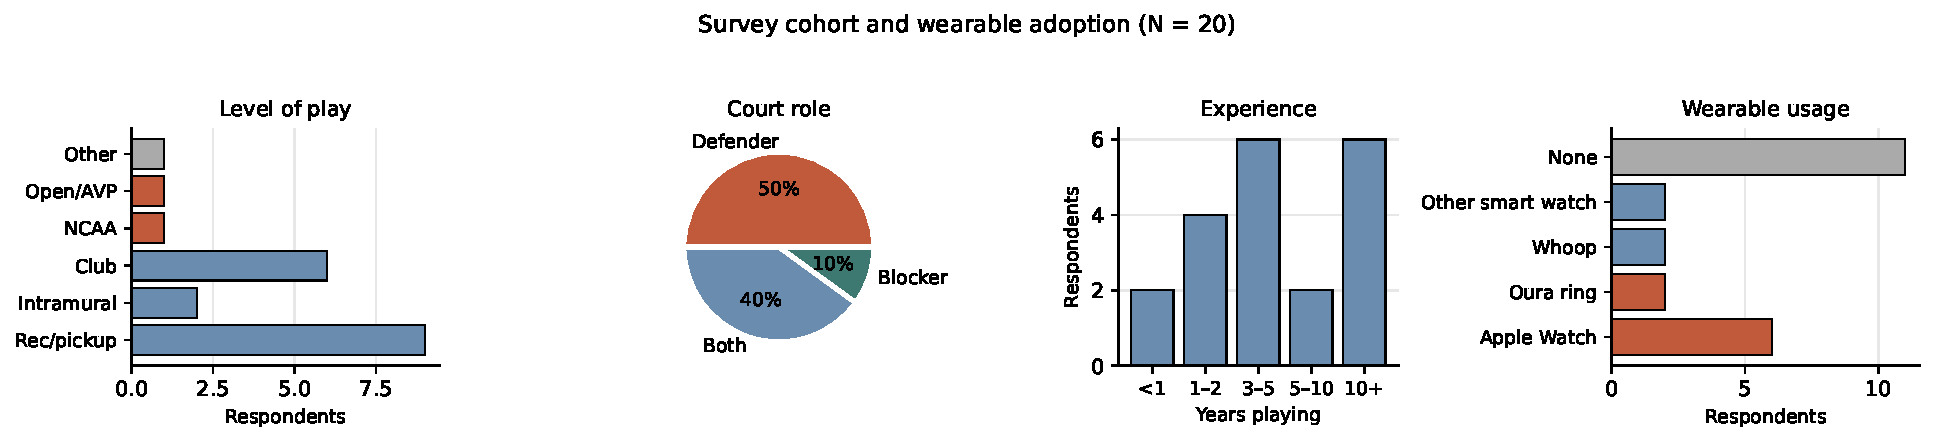
\includegraphics[width=0.93\textwidth]{cohort.pdf}
    \caption{Survey cohort composition and current wearable adoption (N=20). Apple Watch leads existing wearable use (6 of 20), confirming the lead-with-HealthKit decision; Oura and Whoop tie at 2 each.}
    \label{fig:cohort}
\end{figure*}

\begin{figure*}[!htbp]
    \centering
    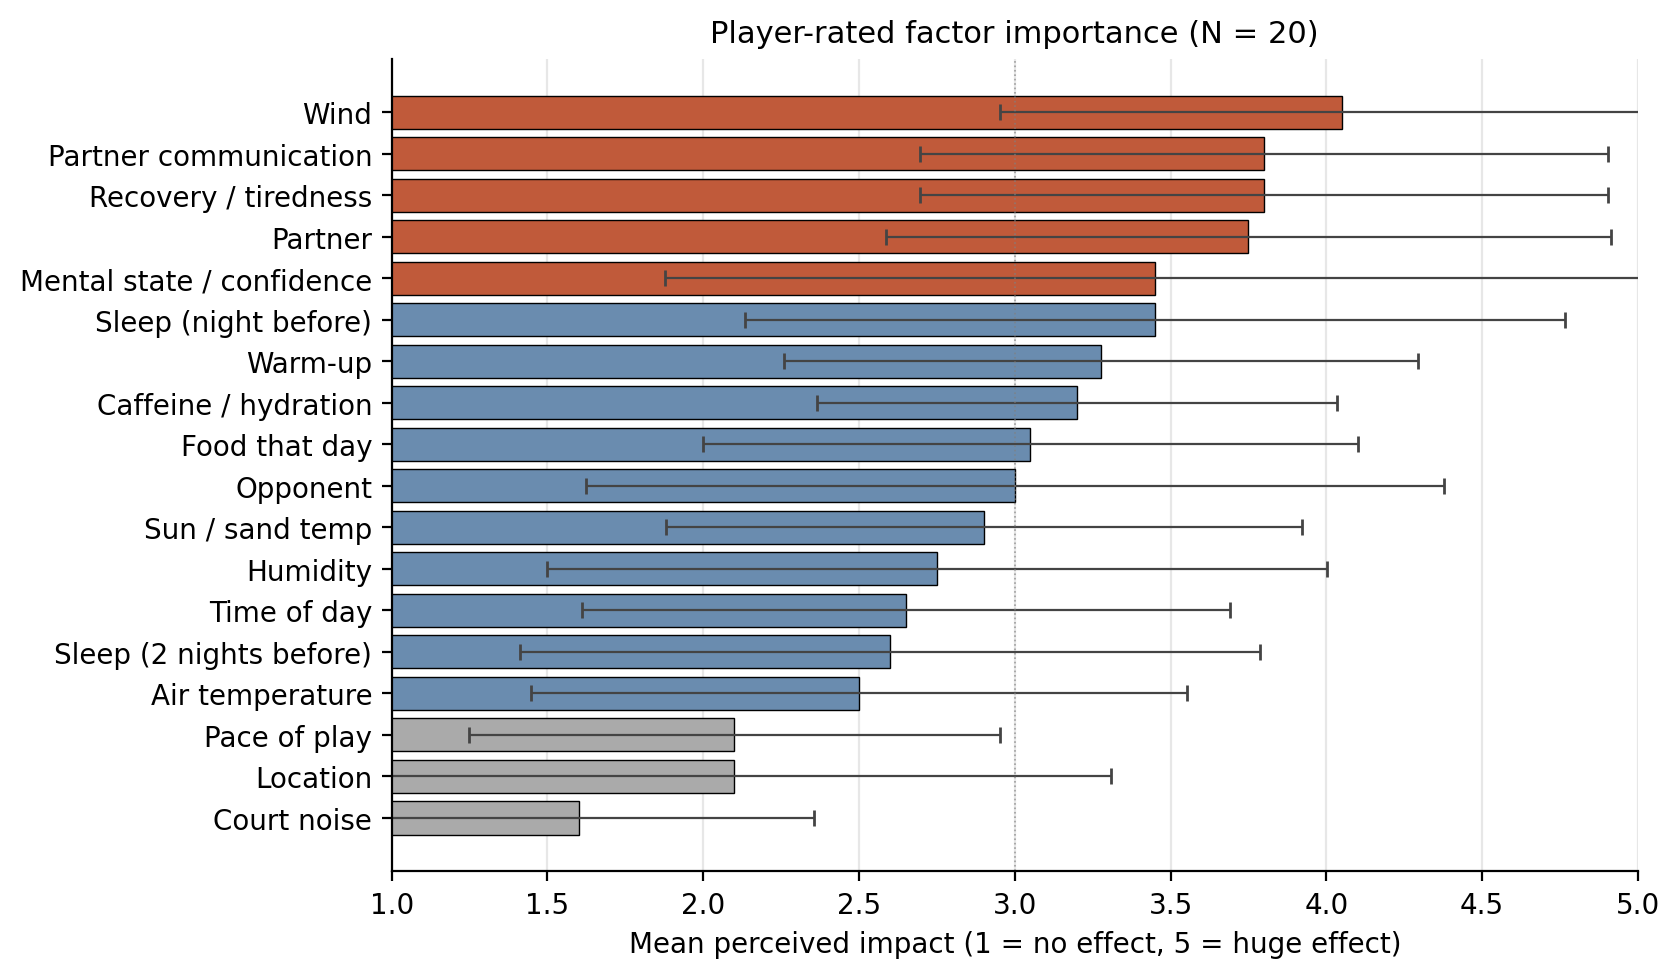
\includegraphics[width=0.78\textwidth]{factor_rankings.png}
    \caption{Player-rated factor importance from the N=20 survey, ordered by mean. Error bars are $\pm 1$ standard deviation. Top five (orange) are retained as primary engineered features; bottom three (gray) have been dropped.}
    \label{fig:survey}
\end{figure*}

Figure~\ref{fig:survey} reports mean perceived importance across 18 candidate factors. The top five (wind, partner communication, recovery/tiredness, partner identity, mental state) all averaged above 3.4/5; three of the five are directly sensable by the current MVP stack. The bottom three (court noise, location, pace of play) all averaged below 2.2/5 and have been dropped from the feature plan. Critically, \textbf{wind ranked first overall} (4.05/5), validating the hardware decision to prioritize wind sensing despite its complexity. Across the cohort, 85\% indicated positive interest in the proposed tool (15\% ``yes, definitely''; 70\% ``maybe, depends on how it works''), with qualified interest concentrated on integration with existing wearables and minimization of in-session burden.

\subsection{Synthesized Player Written Feedback (AI-summarized)}

Open-ended responses surfaced themes not captured in structured ratings. \textbf{Food timing} was the most volunteered factor, with multiple respondents describing large performance swings tied to whether and what they ate in the hour before playing. \textbf{Injury and accumulated soreness} were raised by competitive-level respondents as day-of body-feel distinct from long-term injury status. \textbf{Warm-up quality} appeared independently of the structured rating, suggesting the pre-session ritual may be a useful feature distinct from overall recovery. \textbf{Time-since-last-played} and \textbf{partner attitude/opponent gender} appeared in several responses as factors not anticipated in the original feature list. Qualified ``maybe'' responses converged on three concerns: integration with existing wearables, near-zero in-session burden, and a value proposition centered on controllable factors (sleep, hydration, food) rather than uncontrollable ones (wind, opponent). Two respondents cautioned that over-tracking could cause overthinking --- a useful constraint for any future deployed UI. \emph{This subsection's prose was generated by an AI assistant (Claude) from raw open-ended responses; structured ratings above were unedited.}

%===================================================================
\section{Remaining Goals and Blockers}
%===================================================================

\textbf{This week:} first instrumented data collection at team practice Friday, partner consent finalized, MLX90614 integration on arrival. \textbf{Weeks 8--9:} ramp to two sessions per week, lock the dataset after $\geq 6$ sessions, run the full analysis pipeline, implement HealthKit export. \textbf{Stretch (Weeks 9--10):} voice EMA via Whisper+LLM, partner communication sentiment, MEMS-microphone wind upgrade with anemometer calibration, CV outcome via BalltimeAI. \textbf{Blockers:} the collegiate beach season ended before hardware was operational, pushing first session to Friday; IR sensor lead time delayed sand-temperature integration (DS18B20 closes the gap); BalltimeAI access remains uncertain (\textit{attempting to get free access from my USAVB coach} - CV outcome will be dropped with a limitation paragraph if unresolved by Week 8, per TA feedback). Project is on track for the Week 10 final deliverable.

%===================================================================
\section{AI Use Disclosure}
%===================================================================

AI tools (Claude) were used to (1) generate the prose summary of open-ended survey responses in Section 4.1, as disclosed inline; (2) refine body prose; and (3) render Figure~\ref{fig:arch} from the author's design sketch. All hardware integration, data collection methodology, statistical analysis choices, code, and underlying survey response data are the author's own.\\

\textit{Note exceeded 2 page limit due to many figures included.}


\end{document}